\documentclass[11pt,a4paper,twoside]{article}

\usepackage[utf8]{inputenc}
\usepackage[T1]{fontenc}
\usepackage[english]{babel}
\usepackage{graphicx}
\usepackage{latexsym,amsmath,amssymb,amsthm}
\usepackage{makeidx}
\usepackage[usenames,dvipsnames]{color}
\usepackage[unicode=true,colorlinks=true,linkcolor=RoyalBlue,citecolor=RoyalBlue]{hyperref}
\usepackage{natbib}
\usepackage{lipsum}

\title{The Feed Forward Neural Network library}
\author{Francesco Calcavecchia}

\makeindex

\newcommand{\MRTWO}{$ \text{M}(\text{RT})^2 \;$}
\newcommand{\actf}{\text{a}_f}
\newcommand{\logaf}{\sigma_{\text{lgs}}}
\newcommand{\gssaf}{\sigma_{\text{gss}}}
\newcommand{\idaf}{\sigma_{\text{id}}}


\begin{document}
\maketitle

FFNN (Feed Forward Neural Network) is a C++ library which allows the implementation of a feed forward neural network with few simple calls.
By itself it does not allow for training, but it can be easily combined with the NoisyFunMin library (https://github.com/francesco086/NoisyFunMin) to do so.
The library currently support the evaluation of the NN value, its first and second derivatives in respect to the input, and the first derivative in respect to the variational parameters within the FFNN.

The code has been developed using the standard C++11.

In the following we will present the classes made available by the library.
At the beginning we will report the necessary \verb+#include+ call and the prototype of the class.
The comment \verb+TO DO+ indicates that the method needs to be implemented (as in the case of a pure virtual class).


\section{FeedForwardNeuralNetwork}
\label{sec:NoisyFunction}

\begin{verbatim}
// #include "FeedForwardNeuralNetwork.hpp"
class FeedForwardNeuralNetwork
{
   // Constructor and destructor
   FeedForwardNeuralNetwork(const int &insize,
         const int &hidlaysize,
         const int &outsize);
   FeedForwardNeuralNetwork(const char * filename);
   ~FeedForwardNeuralNetwork();

   // Getters for the basic information
   int getNHiddenLayers();
   int getNLayers();
   int getLayerSize(const int &li);
   ActivationFunctionInterface *
         getLayerActivationFunction(const int &li);

   // Getters for the variational parameters
   int getNBeta();
   double getBeta(const int &ib);
   void setBeta(const int &ib, const double &beta);

   // Set the structure of the FFNN
   void pushHiddenLayer(const int &size);
   void popHiddenLayer();
   void setLayerSize(const int &li, const int &size);
   void setGlobalActivationFunctions(
         ActivationFunctionInterface * actf);
   void setLayerActivationFunction(const int &li,
         ActivationFunctionInterface * actf);

   // Set the computations required
   void addFirstDerivativeSubstrate();
   void addSecondDerivativeSubstrate();
   void addVariationalFirstDerivativeSubstrate();
   void addCrossFirstDerivativeSubstrate();

   // Connect the FFNN,
   void connectFFNN();
   void disconnectFFNN();

   // Set the input
   void setInput(const int &n, const double * in);

   // Feed Forward propagate the input signal
   void FFPropagate();

   // Get the ouput after the FFNN Propagation
   double getOutput(const int &i);
   double getFirstDerivative(const int &i,
                             const int &i1d);
   double getSecondDerivative(const int &i,
                              const int &i2d);
   double getVariationalFirstDerivative(const int &i,
                                        const int &iv1d);
   double getCrossFirstDerivative(const int &i,
                                  const int &i1d,
                                  const int &iv1d);

   // Store the FFNN structure on a file
   void storeOnFile(const char * filename);
};
\end{verbatim}

A \verb+NoisyFunction+ implements a function $f:\mathbb{R}^{n} \rightarrow \mathbb{R} \times \mathbb{R}$ which takes a multidimensional vector as input, and returns a scalar value with an associated error bar.

Fig. \ref{fig:FFNN} illustrates the structure of a Feed Forward Neural Network (FFNN).
A FFNN has always at least one \emph{hidden layer}, an \emph{input layer}, and an \emph{output layer}.
Each layer is made of at least one \emph{unit} (in the figure, the empty circles containing a label) plus an \emph{offset unit} (in the figure, the filled circles).
The number of units in a layer (including the offset unit) is called \emph{layer size}.
Each unit contains a value, labeled with the symbol $u^l_i$, where $l$ is the layer index and $i$ the unit index.
The units with index $i=0$ are not reported in the figure, but represent the offset units.
The units are connected through a net of connections, parametrised by a value $\beta^{l,p}_n$, where $l$ is the index of the layer where the connections are ending, $p$ refers to the index of the origin-unit, and the index $n$ to the index of the destination-unit.

\begin{figure}[htpb]
  \centering
    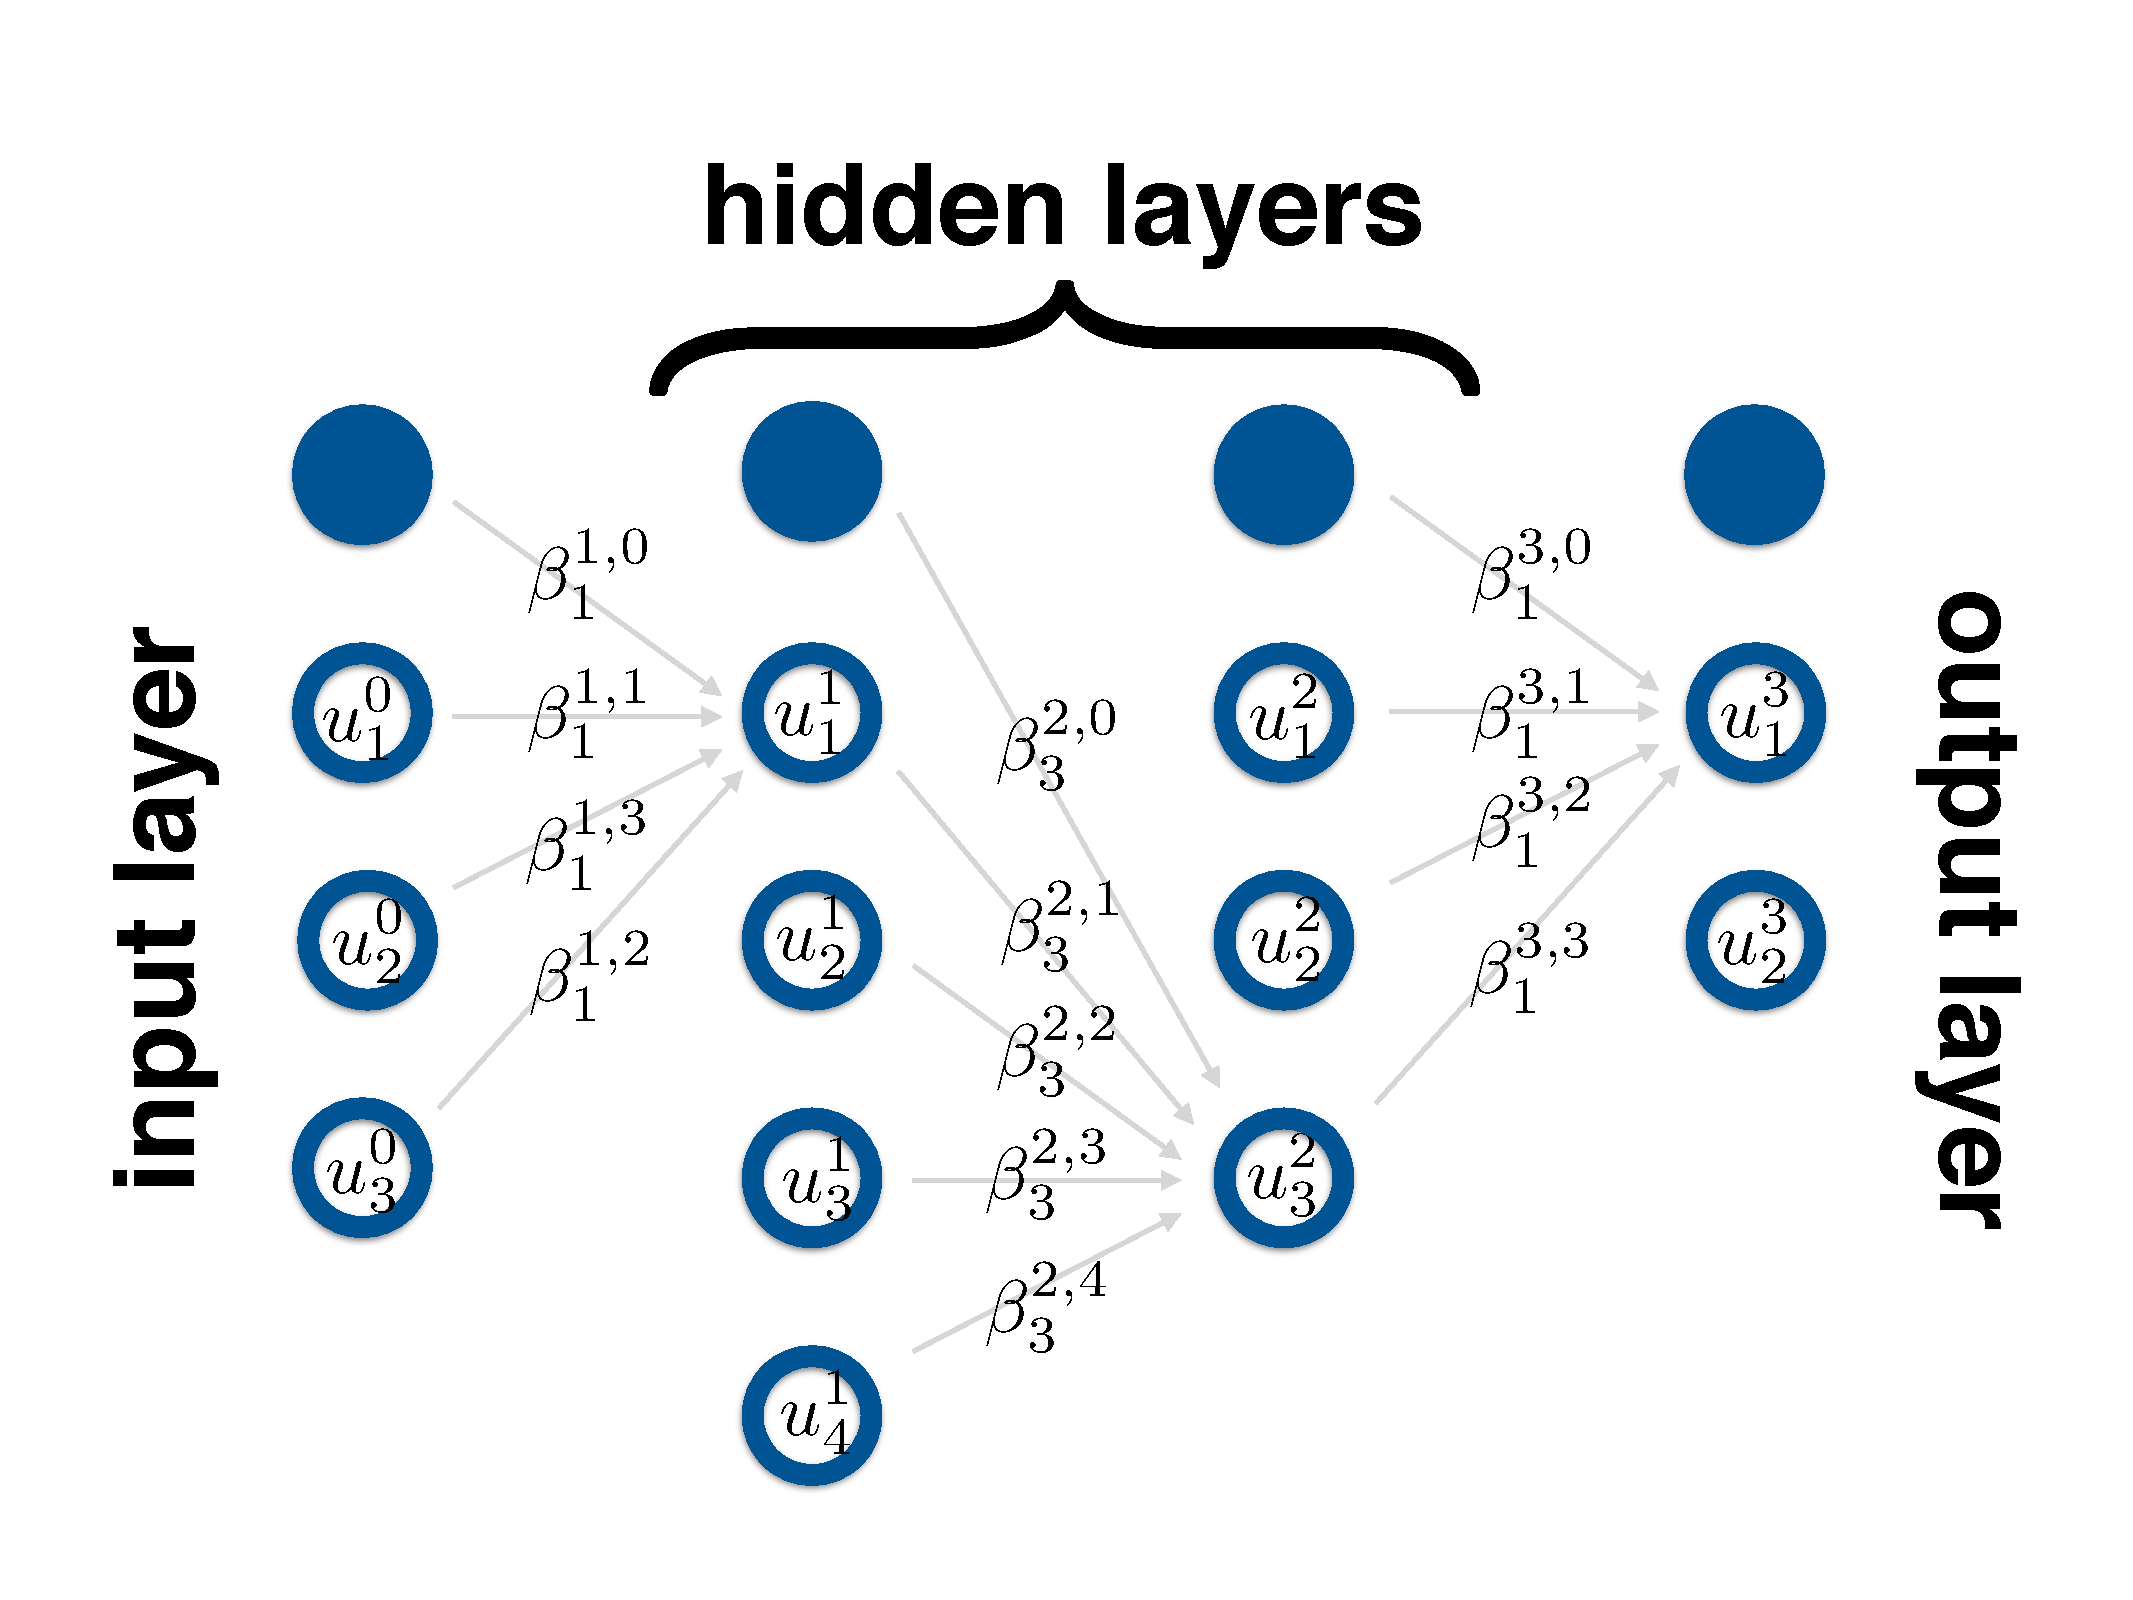
\includegraphics[width=.9\textwidth]{FFNN.pdf}
  \caption{Graphical representation of a Feed Forward Neural Network (FFNN). For a sake of clearness, only some connections are displayed.}
  \label{fig:FFNN}
\end{figure}

Despite the complex tasks that a FFNN can be used for, the math of a FFNN is extremely simple.
A FFNN can be interpreted as a function $f_H: \mathbb{R}^N \rightarrow \mathbb{R}^M$, where $N$ is the size of the input layer (i.e. its number of units, without counting the offset unit), and $M$ the size of the output layer.
The label $H$ represents the number of hidden layers of the FFNN.
Then, once that all the parameters $\beta$ are set, the FFNN output can be computed with the recursive formula:
\begin{equation}
   u^l_i = \actf( u^{l-1}_{k} \beta^{l,k}_{i}  )
\end{equation}
where $\actf: \mathbb{R} \rightarrow \mathbb{R}$ is a so-called \emph{activation function} and we have made use of the Einstein notation, for which repeated symbols on different levels imply a summation, e.g. $x_i^j y^i = \sum_i x_i^j y^i$.
The activation function is required to account for non-linear effects.
The FFNN library provides three activation functions by default, but the user has the possibility to define and use its own, even though its storage on a file it is not supported (explained later).
These three activation functions are:
\begin{enumerate}
   \item the \emph{logistic function}: $\logaf(x) \equiv \frac{1}{1+e^{-x}}$;
   \item the \emph{gaussian}: $\gssaf(x) \equiv e^{-x^2}$;
   \item the \emph{identity}: $\idaf(x) \equiv x$. This function is linear and therefore should not be used normally, but it can be useful in some special circumstances.
\end{enumerate}
By default the logistic function is used for all connections.

The use of the FFNN library should be organised in four major steps:
\begin{enumerate}
   \item generate the geometry of the FFNN;
   \item add substrates, required for computing the derivatives, if necessary;
   \item connect the FFNN;
   \item set the input and propagate it through the FFNN in order to get the output.
\end{enumerate}

Now that the notation of the FFNN has been introduced, and we have briefly seen its structure and math, let us see the methods of this class:
\begin{itemize}
   \item \verb+FeedForwardNeuralNetwork+: There are two possible constructors. The first one takes $3$ \verb+int+, which represents the size of the input, hidden (only one), and output layers. The user can change its shape later on. The values of $\beta$ will be set to some random values. The second constructor takes the path to a file where a FFNN has been stored;
   \item \verb+getNHiddenLayers+: Return the number of hidden layers $H$;
   \item \verb+getNLayers+: Return the total number of layers, i.e. $H+2$;
   \item \verb+getLayerSize+: Return the size of the layer \verb+li+. Remember that $\verb+li+=0$ is reserved for the input layer and $\verb+li+=H+1$ for the output layer;
   \item \verb+getLayerActivationFunction+: Return a pointer to the activation function used to obtain the layer \verb+li+. In the next section we will present the class \verb+ActivationFunctionInterface+;
   \item \verb+getNBeta+: Return the total number of $\beta$;
   \item \verb+getBeta+: Return the value of the $\beta^{l,p}_n$ corresponding to the \verb+ib+:
   $$
   {\verb+ib+} = {\verb+p+} + ({\verb+n+}-1) \, \verb+getLayerSize+({\verb+l+}-1) + \sum_{i=1}^{{\verb+l+}-1} \, \verb+getLayerSize+(i) \, \verb+getLayerSize+(i+1)
   $$
   \item \verb+setBeta+: Set the value of a beta;
   \item \verb+pushHiddenLayer+: Add an hidden layer of size \verb+size+ between the last hidden layer and the output layer. Notice that all the beta related to this layer will be set randomly;
   \item \verb+popHiddenLayer+: Remove the last hidden layer (the one connected to the output layer);
   \item \verb+setLayerSize+: Set the size of a Layer;
   \item \verb+setGlobalActivationFunctions+: Set a global activation function for all the connections in the FFNN;
   \item \verb+setLayerActivationFunction+: Set the activation function used to generate the layer \verb+li+;
   \item \verb+addFirstDerivativeSubstrate+: Add a substrate that allows for the computation of the first derivatives of the FFNN in respect to the input, i.e. $\frac{\partial u^{H+1}_i}{\partial u^0_i}$;
   \item \verb+addSecondDerivativeSubstrate+: Add a substrate that allows for the computation of the first derivatives of the FFNN in respect to the input, i.e. $\frac{\partial^2 u^{H+1}_i}{\partial {u^0_i}^2}$;
   \item \verb+addVariationalFirstDerivativeSubstrate+: Add a substrate that allows for the computation of the first derivative of the FFNN in respect to the variational parameters $\beta$, i.e. $\frac{\partial u^{H+1}_i}{\partial \beta_{i}}$;
   %\item \verb+addLastHiddenLayerVariationalFirstDerivativeSubstrate+: Add a substrate that allows for the computation of the first variational derivatives of the $\beta$ in the last hidden layer only;
   \item \verb+addCrossFirstDerivativeSubstrate+: Add a substrate that allows for the computation of the cross derivatives of the FFNN in respect to the input and the variational parameters $\beta$, i.e. $\frac{\partial^2 u^{H+1}_i}{\partial \beta_{j} \, \partial {u^0_i}}$;
   \item \verb+connectFFNN+: Connect all the units in the FFNN. After this call it is possible to use the FFNN for computing quantities;
   \item \verb+disconnectFFNN+: Disconnect all the units;
   \item \verb+setInput+: Set the values of the units in the input layer. \verb+n+ is the size of the array \verb+in+, and if it does not suite the size of the input layer an error message will be thrown;
   \item \verb+FFPropagate+: Compute the output values, including the derivatives if the substrates have been set accordingly;
   \item \verb+getOutput+: Get the value of the unit \verb+i+ in the output layer;
   \item \verb+getFirstDerivative+: Get the first derivative of the unit value $u^{H+1}_{\verb+i+}$ in respect to $u^0_{\verb+i1d+}$;
   \item \verb+getSecondDerivative+: Get the second derivative of the unit value $u^{H+1}_{\verb+i+}$ in respect to $u^0_{\verb+i2d+}$;
   \item \verb+getVariationalFirstDerivative+: Get the first derivative of the unit value $u^{H+1}_{\verb+i+}$ in respect to $\beta$ with $\verb+ib+ = \verb+iv1d+$. See \verb+getBeta+ for a definition of \verb+ib+;
   \item \verb+getCrossFirstDerivative+: Get the cross derivative of the unit value $u^{H+1}_{\verb+i+}$ in respect to $u^0_{\verb+i1d+}$ and $\beta$ with $\verb+ib+ = \verb+iv1d+$;
   \item \verb+storeOnFile+: Store the FFNNon a file, making possible to retrieve it later on. If the activation functions have been customised, this procedure will not succeed.
\end{itemize}




\section{ActivationFunctionInterface} % (fold)
\label{sec:activationfunctioninterface}

\begin{verbatim}
// #include "ActivationFunctionInterface.hpp"
calss ActivationFunctionInterface
{
   public:

      // compute the activation function value
      virtual double f(const double &) = 0;

      // first derivative of the activation function
      virtual double f1d(const double &) = 0;

      // second derivative of the activation function
      virtual double f2d(const double &) = 0;
};
\end{verbatim}

The \verb+ActivationFunctionInterface+ is a pure virtual class, which can be used to generate customised activation functions to feed a FFNN.
It is necessary to provide the methods \verb+f+, \verb+f1d+, and \verb+f2d+.
As example we report the class for the logistic function:

\begin{verbatim}
class LogisticActivationFunction: public ActivationFunctionInterface
{
   public:

      double f(const double &in)
      {
         return (1./(1.+exp(-in)));
      }

      double f1d(const double &in)
      {
         double f=this->f(in);
         return (f*(1.-f));
      }

      double f2d(const double &in)
      {
         double f=this->f(in);
         return (f*(1.-f)*(1.-2.*f));
      }
};

\end{verbatim}

% section activationfunctioninterface (end)





\printindex

\end{document}
